\chapter{Presentacion del Problema}

En la práctica se van a presentar los siguientes problemas:
\begin{itemize}
	\item Instalacion del entorno.
	\item Multiplicacion de matrices  (Linux)
	\item Procedimiento de desplazamiento Geometrico (OS X)
\end{itemize}

Estos ejemplos nos permitiran visualizar como funciona en diferentes sistemas operativos (aunque similar kernel) la especificacion OpenCL para ello explicare en que consiste cada uno de los problemas listados anteriormente ademas de explicar como he realizado la instalacion en los diferentes sistemas (Linux y OSx)

\section{Instalacion del entorno}

La instalacion para MacOSx ha sido relativamente sencilla pues las librerias vienen implementadas en el programa implementado por apple Xcode asi que una vez instalado desde la Appstore ya esta listo para su funcionamietno.

Sin embargo cuando nos vamos a otro sistema operativo empiezan los problemas, este ha sido el caso de linux, que aun siendo muy similar a MacOSx, la instalacion en este puede dar problemas por la falta de librerias.

Por suerte Nvidia proporciona una serie de archivos ejecutables (.run) que ayudan a la instalacion de este entorno ademas de incorportar ejemplos 

\section{Multiplicacion de matrices}

Aqui presentare el problema pesado para su ejecucion bajo un dispositivo de computacion (en mi caso una tarjeta grafica) este problema aumentara su talla y los resultados se compararan con una ejecucion de secuencial a fin de evaluar estos resultados.

El problema consiste en:

Dos matrices A y B se dicen multiplicables si el número de columnas de A coincide con el número de filas de B.

\begin{figure}
\centering
\incluyeGrafico[width=1.0\textwidth]{matriz7}
\caption{Explicacion de como se reliza una multiplicacion de matrices}
\label{fig:matrixmul}
\end{figure}



El elemento $C_{ij}$ de la matriz producto se obtiene multiplicando cada elemento de la fila i de la matriz A por cada elemento de la columna j de la matriz B y sumándolos.

En nuestro codigo tenemos que una matriz A y una matriz B se multiplican para dar a una matriz C, para cada una hay uqe especificar la memoria que consumira, ya que es uno dee los problemas en la jerarquia de memoria de OpenCL.

\section{Procedimiento de desplazamiento Geometrico}

En esta parte de la practica he incorporado un ejemplo propuesto por Apple que a mi opinion me ha parecido curioso que consiste en una aplicacion de OpenCL y OpenGL que cuya implementacion comparte memoria de ambas tecnologias.

En particular, OpenCL y OpenGL pueden compartir datos, lo que reduce los gastos generales. Por ejemplo, los objetos de OpenGL y los objetos OpenCL creados a partir de objetos de OpenGL pueden acceder a la misma memoria. Además, GLSL (OpenGL Shading Language) shaders y almendras de OpenCL pueden acceder a los datos compartidos.

Para asegurarse de OpenCL y OpenGL hay que estabalecer ciertos parametros:
\begin{itemize}
	\item Establezcer el programa para hacer todo su cálculo y la representación en la GPU.
	\item Asignar memoria para asegurarse de que los datos se comparten de manera eficiente.
\end{itemize}

Esto mejorará el rendimiento, ya que evitará tener que transferir datos entre el host y la GPU.

\begin{figure}[h!]
\centering
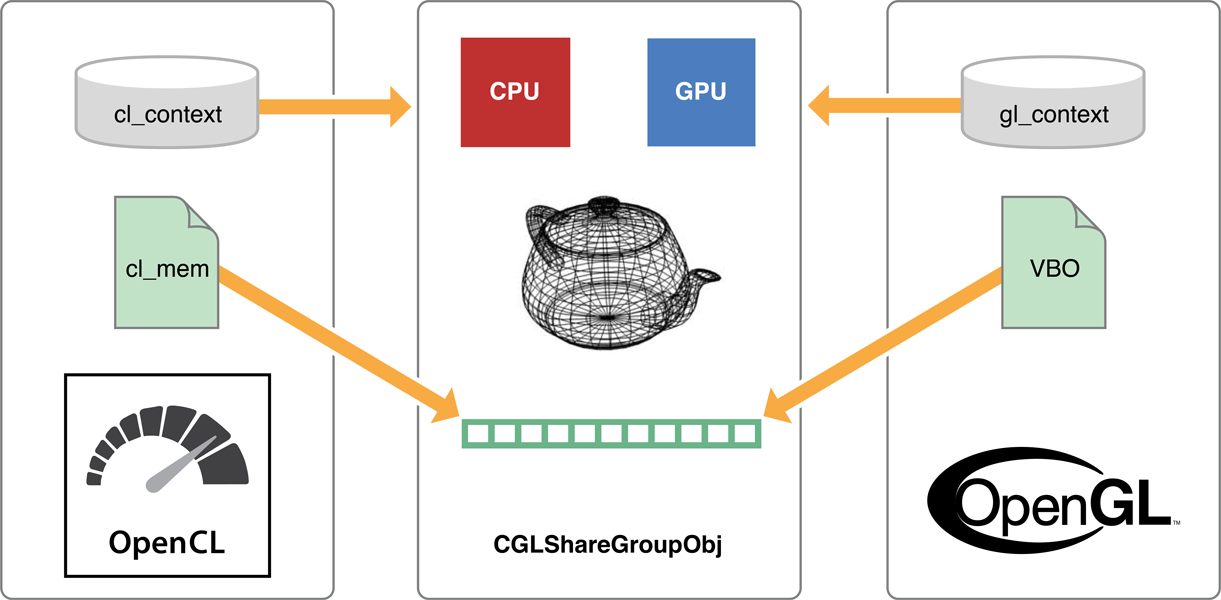
\includegraphics[width=0.7\linewidth]{displacement}
\caption{}
\label{fig:displacement}
\end{figure}

En la  \autoref{fig:displacement} se puede apreciar las dos partes del problema y la solucion compartida, OpenGL genera una imagen y este realiza la carga, mientras que OpenCL se encarga de la gestion de la CPU y la memoria, todo esto nos ofrece una solucion en lo cual se comparte un buffer en el que ambas partes se interconectan.